\documentclass[tikz,border=8pt]{standalone}
\usepackage{amsmath,amssymb}
\usetikzlibrary{arrows.meta,automata,positioning,quotes}
\begin{document}
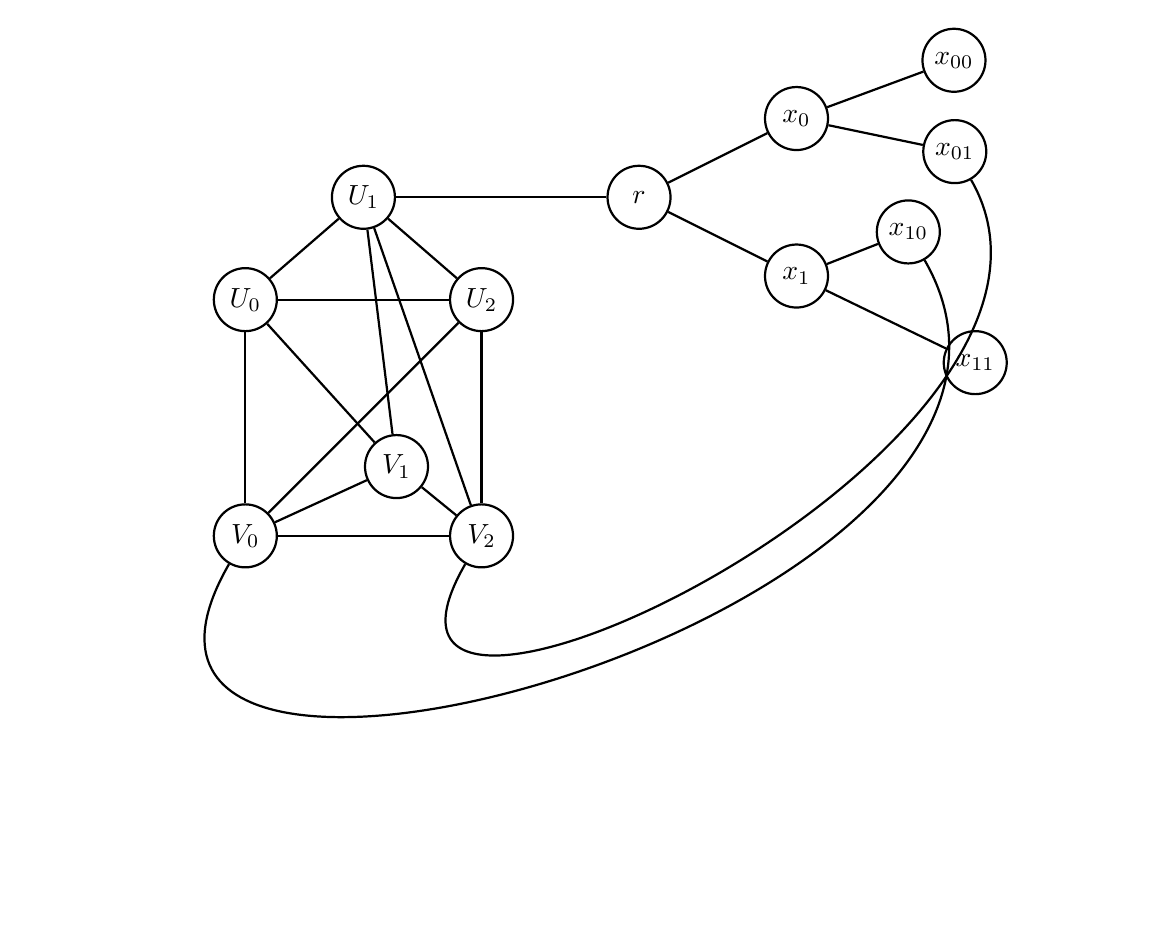
\begin{tikzpicture}[x=1cm,y=1cm]
\tikzset{
  graphnode/.style={circle,draw,thick,minimum size=8mm,inner sep=1pt,font=\sffamily},
  directed/.style={-{Stealth[length=2.4mm]},thick},
  undirected/.style={thick}
}
\node[graphnode] (n_U0) at (-3.00,1.50) {$U_0$};
\node[graphnode] (n_U1) at (-1.50,2.80) {$U_1$};
\node[graphnode] (n_U2) at (0.00,1.50) {$U_2$};
\node[graphnode] (n_V0) at (-3.00,-1.50) {$V_0$};
\node[graphnode] (n_V1) at (-1.08,-0.62) {$V_1$};
\node[graphnode] (n_V2) at (0.00,-1.50) {$V_2$};
\node[graphnode] (n_r) at (2.00,2.80) {$r$};
\node[graphnode] (n_x0) at (4.00,3.80) {$x_0$};
\node[graphnode] (n_x1) at (4.00,1.80) {$x_1$};
\node[graphnode] (n_x00) at (6.00,4.54) {$x_{00}$};
\node[graphnode] (n_x01) at (6.01,3.38) {$x_{01}$};
\node[graphnode] (n_x10) at (5.42,2.36) {$x_{10}$};
\node[graphnode] (n_x11) at (6.27,0.70) {$x_{11}$};
\draw[undirected] (n_U0) -- (n_U1);
\draw[undirected] (n_U1) -- (n_U2);
\draw[undirected] (n_U0) -- (n_U2);
\draw[undirected] (n_V0) -- (n_V1);
\draw[undirected] (n_V1) -- (n_V2);
\draw[undirected] (n_V0) -- (n_V2);
\draw[undirected] (n_U0) -- (n_V0);
\draw[undirected] (n_U1) -- (n_V1);
\draw[undirected] (n_U2) -- (n_V2);
\draw[undirected] (n_U0) -- (n_V1);
\draw[undirected] (n_U1) -- (n_V2);
\draw[undirected] (n_U2) -- (n_V0);
\draw[undirected] (n_U1) -- (n_r);
\draw[undirected] (n_r) -- (n_x0);
\draw[undirected] (n_r) -- (n_x1);
\draw[undirected] (n_x0) -- (n_x00);
\draw[undirected] (n_x0) -- (n_x01);
\draw[undirected] (n_x1) -- (n_x10);
\draw[undirected] (n_x1) -- (n_x11);
\draw[undirected] (n_x01) to[out=300,in=240,looseness=1.25] (n_V2);
\draw[undirected] (n_x10) to[out=300,in=240,looseness=1.35] (n_V0);
\end{tikzpicture}
\end{document}
